%%%%%%%%%%%%%%%%%%%%%%%%%%%%%%%%%%%%%%%%%%%%%%%%%%%%%%%%%%%%%%%%%%%%%%%%%%%%%%

\documentclass{l3deliverable}

%%%%%%%%%%%%%%%%%%%%%%%%%%%%%%%%%%%%%%%%%%%%%%%%%%%%%%%%%%%%%%%%%%%%%%%%%%%%%%

\usepackage{graphicx}%
%
%\usepackage{svn-multi}%
%\svnid{$Id: d3.tex 2500 2011-09-21 15:56:43Z tws $}

\version{1.1 Made  \today  by Ross Eric Barnie}

\usepackage{tabularx}%
\usepackage{url}%
\usepackage{usecasedescription}%

%%%%%%%%%%%%%%%%%%%%%%%%%%%%%%%%%%%%%%%%%%%%%%%%%%%%%%%%%%%%%%%%%%%%%%%%%%%%%%
%% Check these macro values for appropriateness for your own document.

\title{Requirements Document}

\author{Ross Eric Barnie \\
        Dmitrijs Jonins \\
        Daniel McElroy \\
        Murray Ross \\
        Ross Taylor
      }

\date{\today}

\deliverableID{D3}
\project{Team Project 3: Interactive Primer Design}
\team{Q}

%%%%%%%%%%%%%%%%%%%%%%%%%%%%%%%%%%%%%%%%%%%%%%%%%%%%%%%%%%%%%%%%%%%%%%%%%%%%%%

\begin{document}

%%%%%%%%%%%%%%%%%%%%%%%%%%%%%%%%%%%%%%%%%%%%%%%%%%%%%%%%%%%%%%%%%%%%%%%%%%%%%%

\maketitle

\tableofcontents

\newpage

%%%%%%%%%%%%%%%%%%%%%%%%%%%%%%%%%%%%%%%%%%%%%%%%%%%%%%%%%%%%%%%%%%%%%%%%%%%%%%
%% Standard section for all documents

\section{Introduction}

\subsection{Identification}

This document outlines the Requirements Specification of the
Interactive Primer Design system required by the clients. See section
\ref{sec:extendedDefinition} for the definition of the problem the
system will solve.

\subsection{Related Documentation}

% NEED RELATED DOCUMENTATION

%Initial Problem Specification:
%\begin{itemize}
%\item{See section \ref{sec:clientMeetingDocs}} %Attach this if possible
%\end{itemize}

PCR Design Principles (Summary of Meeting on 10/10/2012)
\begin{itemize}
\item{See section \ref{sec:clientMeetingDocs}} 
\end{itemize}

List of Animations Involving PCR Provided by Clients
\begin{itemize}
\item{\url{http://www.youtube.com/watch?v=XXkG6m3yT1M&feature=youtu.be}}
\item{\url{http://ibls.moodle.gla.ac.uk/mod/resource/view.php?inpopup=true&id=33097}}
\item{\url{http://learn.genetics.utah.edu/content/labs/pcr/}}
\end{itemize}

\subsection{Purpose and Description of Document}

This document will serve as an agreement between the client and Team
Q as to the requirements of the system. Any disagreement between the
two parties regarding these requirements will be documented here along
with details on how this was resolved.

\subsection{Document Status and Schedule}

Currently this document is in draft and scheduled to be finalised
pending review and approval from the clients on 7th November 2012.

The next draft of this document (version 1.1) will include all notes from group
meetings and client meetings taken by Team Q and will be included in
appendix \ref{sec:clientMeetingDocs}.
Any changes requested by the clients will also be added for this version.

After which the document will be updated iteratively as changes
arise and will be re-approved by the clients before being re-released.

\section{Extended Problem Defintion}
\label{sec:extendedDefinition}

%%%%%%%%%%%%%%%%%%%%%%%%%%%%%%%%%%%%%%%%%%%%%%%%%%%%%%%%%%%%%%%%%%%%%%%%%%%%%%

Molecular Biology students are required to learn PCR and Primer design
techniques as part of their 3rd year curriculum. 
This system being designed will allow students to use the application
to test their knowledge of these concepts. 
Users will access the NCBI database and copy and paste a gene sequence
into the application. 
The system will then tell them if this is the correct sequence. 
Users will then be asked to select which part of the DNA sequence they
would like to incorporate in the final PCR product.
Once this has been selected, they shall pick a forward and reverse
primer. 
Once these have been selected, various help methods will appear to
help the user determine if they have chosen correcty, if not they will
repeat the process. 
Once correct primer pairs have been picked, the melting temperature of
both primers will be calculated and displayed on screen, and validated
against the primer rules.

%%%%%%%%%%%%%%%%%%%%%%%%%%%%%%%%%%%%%%%%%%%%%%%%%%%%%%%%%%%%%%%%%%%%%%%%%%%%%%

\section{System Scope}

The main aim of this system is to act as a teaching tool to aid students
in learning how to design primers for PCR experiments and should be
usable in a teaching environment or by people on their home computers.

It should function as an interactive, step-by-step guide through the
process of PCR design on a DNA sequence of the users choice.
The user is required to access the NCBI website and copy and paste
their choice of DNA sequence into the system.
The system should provide feedback if the user enters incorrect
primers. 
The system should then check if the melting temperatures of the
primers are in the required range.
The user is then given a link to perform primer blast to check if the
primers they have chosen are unique.

The system should also provide the user help with completing each task
by providing relevant rules for each task and giving the user
instructions about how to use websites and resources outwith the system
(NCBI, primer blast etc.).

When the user has provided an appropriate pair of primers the system
will then show an animation of the PCR reaction taking place.

%%%%%%%%%%%%%%%%%%%%%%%%%%%%%%%%%%%%%%%%%%%%%%%%%%%%%%%%%%%%%%%%%%%%%%%%%%%%%%
\section{Activity Diagram}

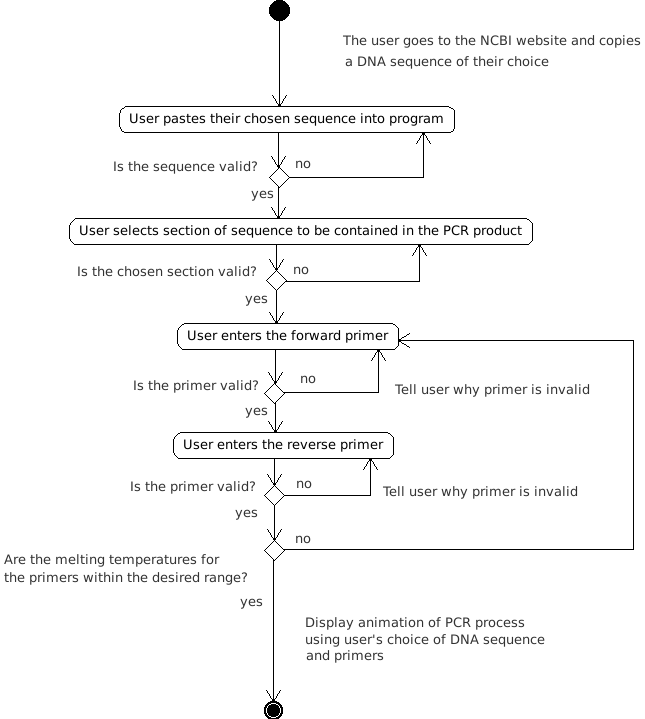
\includegraphics{PCRActivity.png}

%%%%%%%%%%%%%%%%%%%%%%%%%%%%%%%%%%%%%%%%%%%%%%%%%%%%%%%%%%%%%%%%%%%%%%%%%%%%%%

\section{Non Functional Requirements}

%Describe the non-functional requirements for the system here, giving a
%rationale (traceable to your requirements gathering) for each.  You
%will need to think about how to group/structure requirements in this
%section.

\begin{itemize}
\item{
The system is expected to be used at students' homes or in the Biology
lab computers, so portability is essential for the system to work to
the clients' expectations.
}
\end{itemize}

%%%%%%%%%%%%%%%%%%%%%%%%%%%%%%%%%%%%%%%%%%%%%%%%%%%%%%%%%%%%%%%%%%%%%%%%%%%%%%

\appendix

\section{Glossary}
\begin{description}

\item[TP or TP3] {Team Project 3, a compulsory Level 3 Computing
    Science module where students are required to produce some piece
    of software. In our case, this system.}

\item[GitHub] {Refers to the website \url{github.com} which
    hosts the git repository for our project's documentation and
    implentation at \url{https://github.com/Dan-McElroy/Team-Project--Q}}

\item[Git] {A version control system used by Team Q to keep
    track of all digital files related to the system. Not to be
    confused with the term of `endearment' in the English language.}

\item[Portability] {A system which is portable is able to be used on a
    different computer to the one on which it was developed with no,
    or minimal, changes.}

\item[pdf] {A file format used to display documents.}

\item[LaTeX] {A document mark-up language used for all project documentation.}

\item[PCR] {Polymerase chain reaction, a biochemical technology used to amplify pieces of DNA by several orders of magnitude, creating copies of a particular DNA sequence.}

\item[Primer] {A strand that serves as a starting point for DNA synthesis.}

\item[Java] {An object-oriented computer programming language.}

\item[IDE] {An integrated development environment.}

\item[Netbeans] {An IDE for developing primarily in Java.}

\item[Eclipse] {An IDE for developing primarily in Java.}

\item[Swing] {The primary Java GUI widget toolkit.}

\item[JavaFX] {A software platform for creating applications.}

\item[GUI] {Graphical User Interface, an interface which a user interacts with using images.}

\item [PC] {Personal Computer, the terminals which the application will be run on.}

\item [DNA] {Deoxyribonucleic acid, a molecule that contains the genetic instructions used in the functioning of living organisms and many viruses.}

\item [Base] {The a,t,g and c symbols that comprimise a DNA sequence.}

\item [Nucleotide] {Biological molecules that form the building blocks of nucleic acids.}

\item [NCBI] {National Center for Biotechnology Information, a branch of the National Institudes of Health. From their website, users retrieve DNA sequences.}
\end{description}



\section{Client Meeting Documentation}
\label{sec:clientMeetingDocs}

%Any evidence you gathered from stakeholders relevant to your
%requirements description.  You don't need to include everything
%verbatim here, but summary documents, for example, identifying the key
%points you identified (particularly if they relate to requirements
%conflicts) can be useful.

\subsection{Summary of meeting from 10th October 2012}
During the requirements elicitation process, the clients submitted a hand-written document of how they envisioned the system. 

The first two pages contain instructions for how the user would interact with the system, as follows:
\begin{itemize}
\item{Open NCBI}
\item{Type Acc. \# [Accession Number, used to locate the required sequence] into search}
\item{Pull out section of sequence which contains relevant bit for PCR (~500 bases?)}
\end{itemize}
This leads on to a section about primer design, interwoven with diagrams to illustrate their intention. In this document, the plan follows that the user would choose from
a list of 6 potential primers for each strand of the sequence. If the primer chosen is unsuitable, the user will be presented with a clue to inform them why that particular
primer would not be suitable. 
The user would then be prompted to return to the NCBI website, search for the primer sequence using the website's specialised search engine, and if it is unique, 
the system would move on.
The last page contained all the basic rules involved with primer design, which would need to be checked against for the user's choice.

%%%%%%%%%%%%%%%%%%%%%%%%%%%%%%%%%%%%%%%%%%%%%%%%%%%%%%%%%%%%%%%%%%%%%%%%%%%%%%

\end{document}

%%%%%%%%%%%%%%%%%%%%%%%%%%%%%%%%%%%%%%%%%%%%%%%%%%%%%%%%%%%%%%%%%%%%%%%%%%%%%%
